\documentclass{article}

\usepackage[fleqn]{amsmath}
\usepackage{amssymb}
\usepackage{hyperref}
\usepackage{url}
\usepackage{graphicx}
\usepackage{geometry}
\usepackage{babel}
\usepackage{enumitem}
\usepackage{parskip}
\usepackage{chemfig}
\usepackage{pdfpages}
\usepackage{xcolor}
\usepackage{tikz}
\usepackage{fancybox}
\usepackage{makecell}
\usepackage{pgfplots}
\usepackage{soul}
\usepackage{ulem}
\usepackage{wrapfig}
\usepackage{subcaption}
\usepackage[T1]{fontenc}
\usepackage{esvect}
\usetikzlibrary{arrows}
\usetikzlibrary{decorations.pathreplacing}
\pgfplotsset{compat=1.17}

\geometry{
    a4paper,
    total={170mm, 257mm},
    left=20mm,
    top=20mm
}

\hypersetup{
    colorlinks=true,
    linkcolor=black,
    urlcolor=blue,
    pdftitle={System engineering in EES}
}

\newcommand{\figbox}[1]{ 
    \begin{figure*}[ht!]        
        \begin{center}            
            \fbox{#1}        
        \end{center}    
    \end{figure*}
}

\newcommand{\wrapfill}{
    \par
    \ifnum \value{WF@wrappedlines} > 0
        \addtocounter{WF@wrappedlines}{-1}%
        \null\vspace{
            \arabic{WF@wrappedlines}
            \baselineskip
        }
        \WFclear
    \fi
    \phantom{}
}

\newcommand{\cfig}[1]{%
  \begin{figure*}[ht!]%
    \centering%
    #1%
  \end{figure*}%
}

\newcommand{\difference}{\,\backslash\,}
\newcommand{\rem}{\underline{Remark}: }
\newcommand{\nots}{\underline{Notation}: }
\newcommand{\prf}{\underline{Proof}: }
\newcommand{\exs}{\underline{Example}: }
\newcommand{\defs}{\underline{Definition}: }
\newcommand{\wrn}{\underline{Warning}: }
\newcommand{\sht}{\ |\ }


% === TEXT ===
\title{\textbf{Systems Engineering in\\Environmental and Energie Systems\\ HSLU, Semester 1}}
\author{Matteo Frongillo}

\begin{document}

\maketitle
\tableofcontents
\pagebreak

\part{Week 1}

\section{Waste to energy (WtE)}
Waste to energy refers to a variety of treatment technologies that convert waste to electricity,
heat, fuel or other usable materials, as well as a range of residues.

\setlength{\intextsep}{0pt}%
\begin{wrapfigure}{r}{.5\textwidth}
    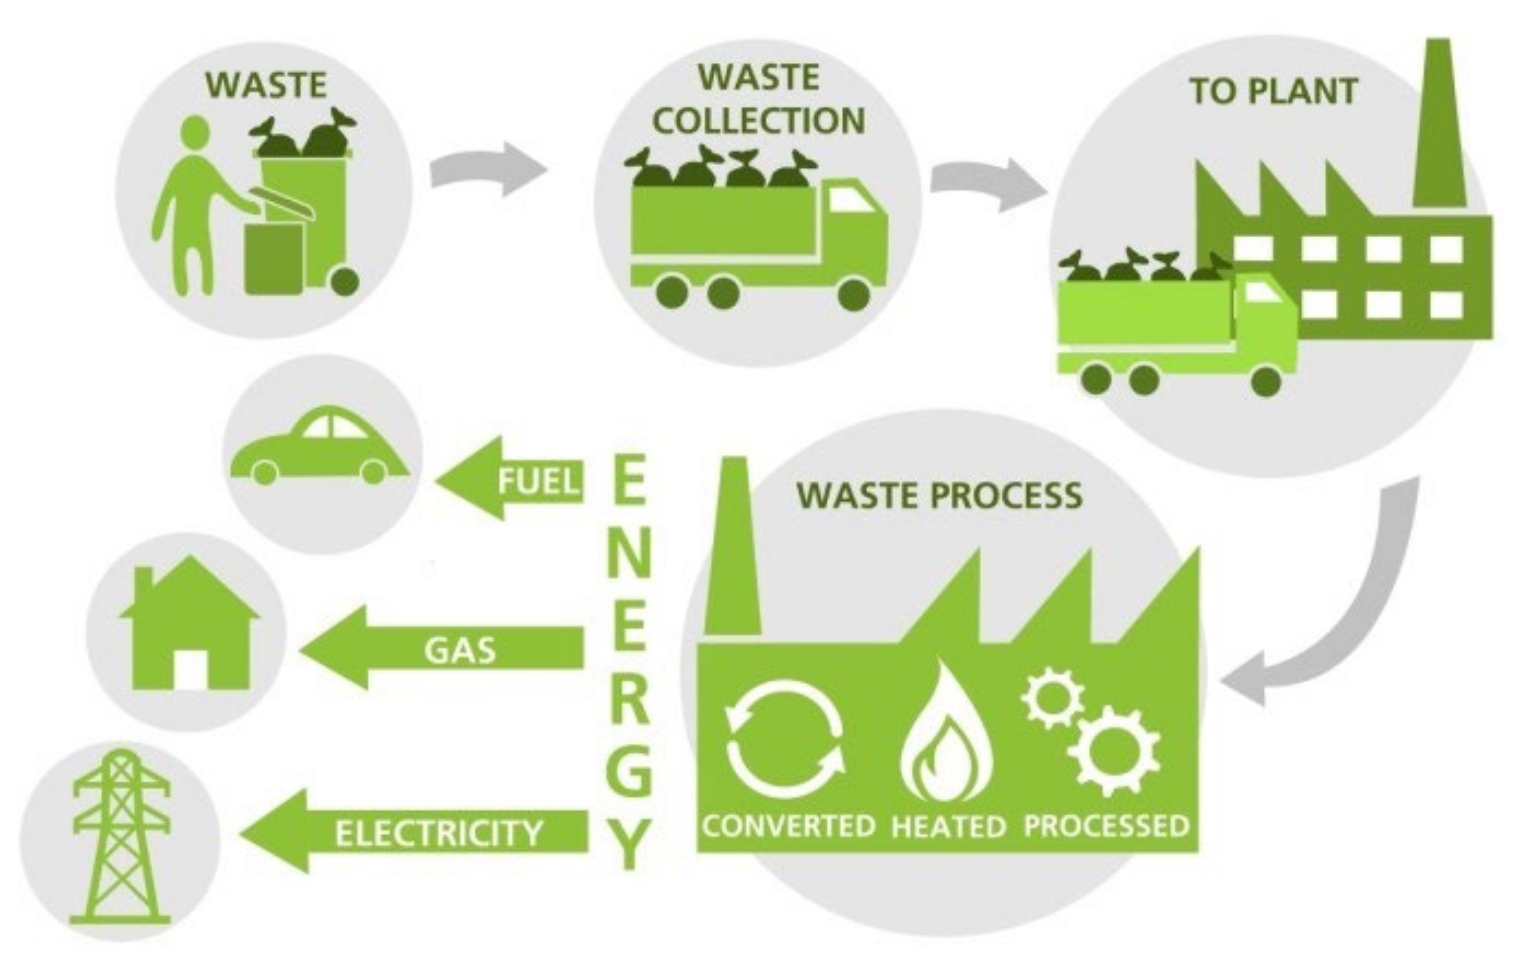
\includegraphics[width=.5\textwidth]{media/WtE.png}
    \vspace{-2.6cm}
\end{wrapfigure}

\phantom{}

WtE can occur through a number of processes\\such as:
\begin{itemize}
    \item incineration;
    \item gasification;
    \item pyrolysis;
    \item anaerobic digestion;
    \item landfill gas recovery.
\end{itemize}
\wrapfill

\subsection{Incineration plants}
Thermal waste to energy, also known as incineration with energy recovery, is a major waste
treatment method and the most widely adopted technology that dominates the global WtE market.

An incineration plant is a waste management facility designed to burn solid waste at high temperatures,
converting in into ash, gases and heat.

Incineration plays a crucial role in modern waste management strategies, contibuting to
environmental protection and resource recovery.

\begin{itemize}
    \item Volume reduction of waste (90\%);
    \item Energy production: waste has the same energy value as wood chips or lignite;
    \item Reduction of contaminant spectrum: bacteria, viruses and problematic organic
        compounds are destroyed at or over 1'000 $^\circ$C;
    \item Low pollutant emissions (modern incineration plants);
    \item Avoidance of methane emissions that results from direct deposition of organic
        waste in landfills;
    \item Chemical stability of residues/slag (compared to biological processes);
    \item Possibility of recovering metals from slag (80kg of iron, 20kg of aluminium and 2kg of copper are recovered per each tonne of slag).
\end{itemize}

\subsubsection{Incineration plants vs. Landfills}
Incinerators can generate more CO$_2$ than landfills for every unit of electricity.
Landfills, on the other hand, produce energy more effectively. However, while
they don't make as much CO$_2$ as waste to energy incineration, they produce methane,
which is stronger greenhouse gas.

Incineration plants are preferred over landfills because incineration can reduce the amount of
waste which must be diverted to landfill by as much as 95\%, which is an efficient method
of dealing with the issue. Incineration alto eliminates the need to transport the waste to other locations
or countries, thus cutting down on the emissions involved in that stage of the proces.


\subsubsection{4-key Components of an incineration plant}
\begin{enumerate}
    \item Waste handling system: responsible for loading, sorting and feeding waste into
        the combustion chamber;
    \item Combustion chamber: primary unit where waste is incinerated at temperature
        between 800 and 1'200 $^\circ$C;
    \item Air pollution control system: filters and scrubbers to minimize harmful emissions
        and comply with environmental regulations;
    \item Energy recovery system: utilizes the generated heat to produce electricity or heat
        for district heating.
\end{enumerate}

\subsubsection{Incineration plant scheme}
\phantom{}
\cfig{\includegraphics*[width=.9\textwidth]{media/incineration-plant-scheme.png}}
\phantom{}

\subsubsection{Waste incineration plants in Switzerland}
There are around 30 incineration plants across Switzerland.

About four million tonnes of combustible waste from Switzerland and abroad
is inciderated to generate thermal energy in municipal incinerators.
The heat generated during combustion is used to produce electricity,
operate district heating networks or as process heat in industrial plants.

In 2017, the 30 municipal incinerators produced a record amount of energy
totalling 4'036 GWh of heat and 2'338 GWh of electricity.

They thus contribute around 2.5\% of Switzerland's total energy requirements
and just under 4\% of the country's overall electricity production.

\subsection{Types of wastes that can be converted into energy}
\subsubsection{Municipal Solid Waste (MSW)}
Municipal wastes can be converted into energy by thermochemical or biological technologies.

At the landfill sites, gasses produced by the natural decomposition of MSW can be collected,
scrubbed and cleaned before feeding into internal combustion engines or gas turbines to
generate heat and power.

The organic fraction of MSW can be biochemically stabilizen in an anaerobic digester to
obtain biogas (for heating and power) as well as fertilizer.

\subsubsection{Wood wastes}
Wood processing industries primarly include sawmilling, plywood, wood panel, furniture,
building component, flooring, particle board, moulding, jointing and craft industries.

Wood wastes generally are concentrated at processing factories (e.g. plywood mills and
sawmills). In general, processing 1'000 kg of wood in the furniture industries, will lead to
waste generation of 45\%.

Similarly, when processing 1'000 kg of wood in sawmill, the waste will amount to more than
half (52\%).

Wood wastes has high calorific value and can be efficiency converted into energy
by thermal technologies, like combustion and gasification.

\subsubsection{Agricultural wastes}
Agricultural wastes include encompasses all kind of crop residues, such as bagasse, straw,
stem, stalk, leaves, hush, shell, peel, pulp, stubble, ...

Large quantities of crop residues are produced annually in the MENA region, and are vastly underutilised.
Dates, wheat and barley are the major staple crops grown in the Middle East region.
In addition, the region has witnessed very rapid growth in the poultry sector.

\subsubsection{Industrial wastes}
The food processing industry in MENA produces a large number of organic wastes and
by-products that can be used as biomass energy sources.

These waste materials are generated from all sectors of the food industry
with everything from meat production to confectionery producing waste that can be utilised
as an energy source. In the recent decades, the fast-growing food and beverage
industry has remarkably increased in importance in major countries of the region.

\subsubsection{Animal wastes}
The MENA countries have strng animal population. The livestock sector, in particular
sheep, goats and camels, plays an important role in the national economy
of respective coutries.

Many millions of live ruminants are imported each year from around the world.
In addition, the region has witnessed very rapid growth in the poultry sector.

\subsubsection{Hazardous waste}
Waste containing toxic chemicals, radioactive materials, or heavy metals can pose serious
environmental and health risks. Burning or processing these materials
can release harmful pollutants.

\subsubsection{Non-combustible materials}
Materials like glass, metals, and ceramics cannot be used for combustion-based
energy recovery, since they don't burn or provide calorific value.

\subsubsection{Electronic wastes (E-waste)}
While some components of e-waste (like plastic) may be combustible, burning electronic
waste can release toxic fumes and should instead be recycled to recover valuable materials like metals.

\subsubsection{Inert construction and demolition waste}
Items like concrete, bricks, and stones are not suitable for energy recovery,
since they do not contain combustible materials.

\subsection{Current status of waste to energy}
IMMAGINE

\subsubsection{Waste production per person in CH}
In Switzerland, people produce 700kg of waste per person per year.

\subsection{Waste hierarchy}
The hierarchy helps us rethink our relationship with waste based on
five priorities ranked in terms of what is best for the environment:

\begin{enumerate}
    \item Produc prevention;
    \item Preparing for re-use;
    \item Recycle;
    \item Recovery;
    \item Waste disposal.
\end{enumerate}

\subsection{Advantages and disadvantages of the Swiss system}
\subsubsection{Advantages}
...

\subsubsection{Disadvantages}
...

\section{System thinking}
\subsection{Benefits}
Rigorous way of integrating: people, purposes, process and performance and:
\begin{itemize}
    \item ...
\end{itemize}

\subsection{Feedback loops}
...

\section{Case study part 1}
...

\part{Week 2}
\section{Situation analysis and system thinking}








\end{document}
